This sections describes the latest iteration of the YOLO detection pipeline. While this network is not specifically designed for detection in remote sensing, it consistently obtains extremely great scores in all datasets. Understanding how this version is able to improve both speed and precsion can help us designing a better network. The article details and experiments with a large number of features, be it training wise or architecture wise to help configure a better YOLO model. In short, this article presents the \textbf{best practices in CNN design}. First the authors describes two different approaches: the "\textbf{Bag of Freebies}" (BoF), where researchers develop better training method to make the detector more accurate without increasing the inference cost. We will summarize those in section\ref{bof}. Another approaches is the one using special modules, that increases the inference cost by a small fractions, but gives out great improvement to the accuracy. This is what the authors calls the "\textbf{Bag of Special}" (BoS), which are described in section \ref{bos}. 


\subsection{General Architecture of a Object Detector}
The authors describes the composition of a modern detector. Those detectors are usually comprised of two parts. First a backbone, usually trained on ImageNet\cite{imageNet} which creates the feature maps from the input image, and secondly a head, which infer bounding boxes and classes. The backbone we are usually interested in, meaning the ones running on GPUs and not CPUs are VGG\cite{vgg}, resNet\cite{resNet}, resNeXt\cite{resNeXt} or DenseNet\cite{denseNet}. We have already seen a few of those backbones in previously reviewed articles, especially resNet.

\begin{figure}[h]
  \centering
  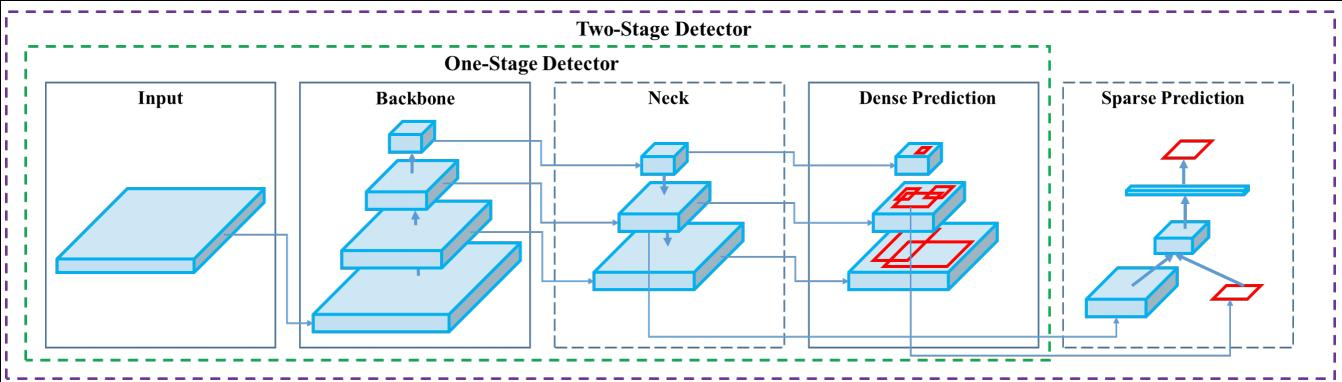
\includegraphics[width=\textwidth]{archiYOLO}
	\caption{General Architecture of an Object Detector}
  \label{fig:genArchi}
\end{figure}
The head part is divided in two categories: one-stage object detectors such as YOLO\cite{yolov9000, yolov3}, SSD\cite{ssd} or RetinaNet\cite{retinaNet}. Examples of two stages detectors are the R-CNNs\cite{rcnn}, like Fast R-CNN \cite{fastRCNN}, Faster R-CNN\cite{FasterRCNN} or R-FCN\cite{rfcn}.

Modern object detectors usually have a layer collecting feature maps from different stages, such as feature fusion modules. The author call this layer the 'neck'. Networks using this type of mechanisms include Feature Pyramid Network (FPN)\cite{fpn}, Path Aggregation Network (PAN)\cite{pan}, BiPFN\cite{bifpn} and NAS-FPN\cite{nasFPN}

To summarize, an object detector is made up of the following parts:

\begin{itemize}
	\item \textbf{Backbones}: VGG\cite{vgg}, ResNet-50\cite{resNet}, EfficientNet\cite{efficientNet}, CSPResNeXt50\cite{resNeXt}, CSPDarknet53\cite{CSPDarknet53}.
	\item \textbf{Neck}:
		\begin{itemize}
			\item \textbf{Additional Blocks}: SPP\cite{spp}, ASPP\cite{aspp}, RFB\cite{RFB}, SAM\cite{sam}
			\item \textbf{Path-aggregation blocks}: FPN\cite{fpn},NAS-FPN\cite{nasFPN} PAN\cite{pan}, BiFPN\cite{bifpn}, ASFF\cite{ASFF}, SFAM\cite{SFAM} 
		\end{itemize}
	\item \textbf{Heads}:
		\begin{itemize}
			\item \textbf{Dense Prediction (One-Stage)}
				\begin{itemize}
					\item Anchor-based: RPN\cite{FasterRCNN}, SSD\cite{ssd}, YOLO\cite{yolov3}, RetinaNet\cite{retinaNet}
					\item Anchor-free: CornerNet\cite{cornerNet}, CenterNet\cite{centerNet}, MatrixNet\cite{matrixNet}, FCOS\cite{fcos}
				\end{itemize}
			\item \textbf{Sparse Prediction (Two-stage)}
				\begin{itemize}
					\item Anchor-based: Faster R-CNN\cite{FasterRCNN}, R-FCN\cite{rfcn}, Mask R-CNN\cite{maskrcnn}
					\item Anchor Free : RepPoints\cite{repPoints}
				\end{itemize}
		\end{itemize}

\end{itemize}

\subsection{Bag of Freebies}\label{bof}
This section presents training techniques to improve detection rates without increasing the inference costs. Most of those techniques that falls under this definition are data augmentation methods. Data augmentation aims to increase the variability of the training images, so that the model will be more robust. Commonly used techniques are photometric distortions, where the brightness, contrast, hue and saturation of an image is adjusted, or geometric distortion, with random rescaling, cropping, flipping and rotating.

Those techniques are pixel-wise adjustments, meaning that the original pixel information in the adjusted area is retained. Novel data augmentation techniques have an emphasis put in object occlusion issues. Random Erase\cite{randomErase} or CutOut\cite{cutOut} randomly selects a rectangle region in an image and fills with random values. Hide and seek\cite{hideSeek} and grid mask\cite{gridMask} randomly selects multiple rectangle regions in an image and replaces them to all zeros.  Similar techniques are applied to feature maps, for example, DropOut\cite{dropOut}, DropConnect\cite{dropConnect} and DropBlock\cite{dropBlock}.

Other methods uses multiple image together. MixUP\cite{mixUp} uses two images to multiply and superimpose them with different coefficient ratios, and adjusts the labels with these ratios. CutMix\cite{cutMix} crops an image and cover another images with this cropped region, adjusting the labels according to the size of the covered area.

\begin{figure}
     \centering
     \begin{subfigure}[b]{0.3\textwidth}
         \centering
         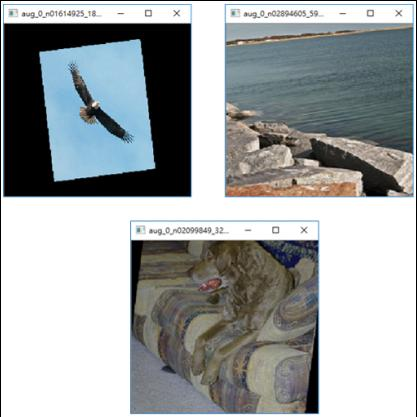
\includegraphics[width=\textwidth]{dataAugmA}
         \caption{Classic image data augmentation: crop, rotation, flip, hue, saturation, brightness}
         \label{fig:classicAugm}
     \end{subfigure}
     \hfill
     \begin{subfigure}[b]{0.3\textwidth}
         \centering
         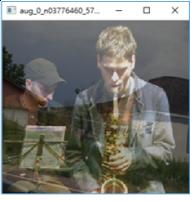
\includegraphics[width=\textwidth]{dataAugmB}
         \caption{MixUp}
         \label{fig:mixup}
     \end{subfigure}
     \hfill
     \begin{subfigure}[b]{0.3\textwidth}
         \centering
         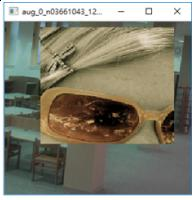
\includegraphics[width=\textwidth]{dataAugmC}
         \caption{CutMix}
         \label{fig:cutMix}
     \end{subfigure}
        \caption{Some data augmentation techniques}
        \label{fig:dataAugm}
\end{figure}


Even StyleTransfer GANs\cite{styleTransfer} have been used for data augmentation, reducing the texture bias learned by CNN.

Other data augmentation techniques have been focussed in reducing the amount of bias present in the semantic distribution of the dataset. For example, there might be a problem of data imbalance between different classes, which can be solved by hard negative example mining\cite{hardNegMining} or online hard example mining\cite{onlineHard} in two-stage object detectors. However these example mining methods are not applicable in one-stage object detectors. For those detectors, focal loss\cite{focalLoss} have been proposed to deal with the problem of data imbalance. 

Another issue is that it is difficult to express the relationship of the degree of association between different categories with the one-hot representation, often used when executing labeling. Label smoothing\cite{labelSmooth} convert hard label into soft label, which can make the model more robust. Knowledge distillation have also been used to design a label refinement network.\cite{knowledgeDistillation}.

Finally, the objective function for the bounding box have also been the focus of improvements. Usually, Mean Square Error (MSE) have been used to perform regression on the center point coordinates, height and width of the Bounding Box. However, to directly estimate the coordinates of the bounding box is to treat those points as independent variables, which \textbf{does not consider the integrity of the object itself}. The IoU loss\cite{iouloss} puts the coverage of the predicted bounding box area and the ground truth area into consideration. GIoU loss\cite{giou} is an improvement on this loss, and also include the shape and orientation of the object in addition to the coverage area\footnote{An improvement to this has been done for automated detection in satellite imagery by Qian and Al and is covered in section \ref{qianAl}}. Finally, DIoU loss\cite{diou} also considers the distance of the center of an object and CIoU\cite{diou} considers the overlapping area, the distance between center points and the aspect ratio.

\subsection{Bag Of Specials}\label{bos}
Other methods that improve the detection rate at the expense of a small increase in inference cost are what the authors refers to as "Bag of Specials" (BoS). Those methods are generally plugin modules that enhance certain attributes of the model. For example, they can enlarge the receptive field, introduce an attention mechanism or strengthen the feature integration capability.

Common modules uses to improve the receptive field are SPP\cite{spp}, ASPP\cite{aspp} and RFB\cite{RFB}. The SPP originates from Spatial Pyramid Matching (SPM) \cite{SPM}. SPM method is to split the feature maps into several $d \times d$ blocks of equal size, where $d$ can be ${1, 2, 3,...}$. This forms spatial pyramids, where we can then extract bag-of-words features. SPP integrate SPM into a CNN, and uses the max-pooling operation instead of bag-of-word. However, this SPP module output one dimensional feature vectors, which makes it inapplicable for Fully Convolutionnal Network (FCN). In YOLOv3\cite{yolov3}, the SPP module is improved by concatenating the max-pooling outputs with kernel size $k \times k$ with $k = \{1, 5, 9, 13\}$ and stride of 1. This modules improves the YOLOv3 $AP_{50}$ by 2.7\% on the MS COCO\cite{msCOCO} datasets for only  0.5\% extra computation. 

Attention is also used to improve the capabilities of detection networks. Attention modules are divided in two categories: channel-wise attention, with the Squeeze-and-Excitation (SE)\cite{squeezeExcite} and point-wise attention with Spatial Attention Module (SAM) \cite{sam}. SE modules can improve the accuracy of ResNet by 1\% in the ImageNet\cite{imageNet} dataset, however this comes at in increase of inference time of 10\% on a GPU. In comparison, SAM only demands 0.1\% extra calculation but improve the ResNet50 top-1 accuracy by 0.5\%. This module does not affect the inference speed.

Feature integration modules allows the model to take into account features computed from earlier layers. Early examples are skip connections\cite{skipCo} or hyper-column\cite{hyperColumn} integrate low-level physical and geometric features to high-level semantic feature. Now, lightweights modules that integrates different feature pyramids are used, like SFAM\cite{SFAM}, ASFF\cite{ASFF} and BiFPN\cite{bifpn}. The idea behind SFAM is to use SE modules to execute channel-wise re-weighting on multi-scale concatenated feature maps. ASFF uses softmax as point-wise level re-weighting and adds feature maps of different scales. In BiFPN multi-input weighted residual connections is used to execute scale-wise level re-weighting, and then add feature maps of different scales.

A good activation function is crucial to correctly train a network, and much work has been put into trying to design a better one. In 2010, ReLU\cite{relu} was proposed as a solution to vanishing gradient problem. Offshoots, such as LeakyRelu\cite{leakyRelu}, PReLU\cite{prelu}, ReLU6\cite{mobileNet}, Scale Exponential Linear Unit (SELU) \cite{selu}, Swish \cite{swish}, hard-Swish\cite{hswish} and Mish\cite{mish} have been proposed. LReLU and PReLU serves to solve the problem that the gradient of ReLU is zero when the output is less than 0. ReLU6 and hard-swish are specially designed for quantization networks. The SELU activation function tries to self-normalize a neural network. Swish and Mish are continuously differentiable.

Post-processing with NMS is usually done with detection network to remove superfluous bounding boxes and only retain the ones with the highest response. However NMS does not consider contextual information, so Girshick \textit{et al.}\cite{girshick2013} added classification confidence scores in R-CNN as a reference. Soft NMS\cite{softNMS} considers the problem that occlusion of an object may cause the degradation of confidence score in greedy NMS with IoU score. DIoU NMS\cite{diou} adds the information of the center point distance to bounding box. 

\subsection{Additional Improvements}
\textbf{The main goal of this architecture is to make the detector suitable for training on a single consumer-grade GPU so additional design improvements were made}. First, new methods of data augmentation are used: Mosaic and Self-Adversarial Training. Optimal hyper-parameters were chosen using genetic algorithms. Finally, modifications were made to existing methods to make them more efficient for training and detection, namely SAM, PAN and Cross mini-Batch normalization.

\begin{figure}[H]
  \centering
  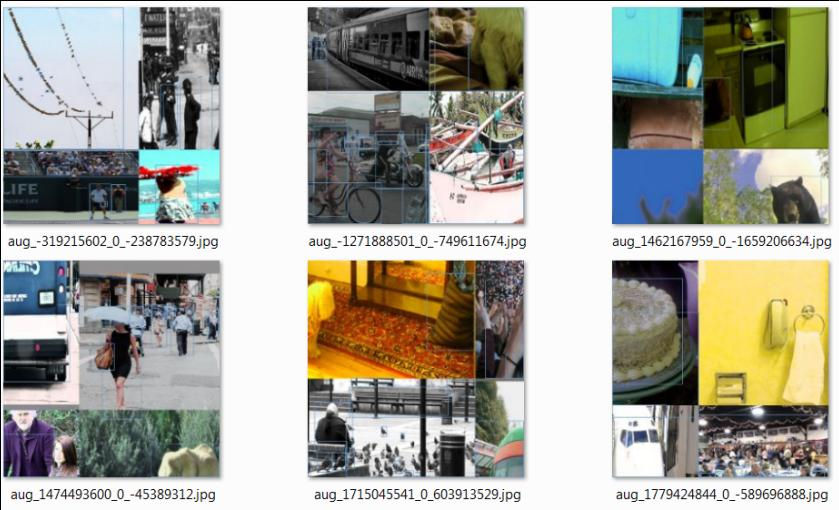
\includegraphics[width=0.7\textwidth]{mosaic}
	\caption[]{The Mosaic data augmentation technique}
  \label{fig:mosaic}
\end{figure}

\textbf{Mosaic is a new data augmentation method that mixes 4 training images so that 4 different context are mixed}, and is shown in Figure~\ref{fig:mosaic}. This allows detection of objects outside their normal context. Batch normalisation calculates activation statistics from 4 different images on each layer, which significantly reduces the need for a large mini-batch size.

Self-Adversarial Training operates in 2 forward-backward stages. In the 1st stage, the neural network alters the original image instead of the network weights. \textbf{This way, the network executes an adversarial attack on itself, altering the original image and making it look like there is no object to detect}. In the 2nd stage, the network is trained to detect an object on this modified image in the normal way.

\begin{figure}[H]
  \centering
  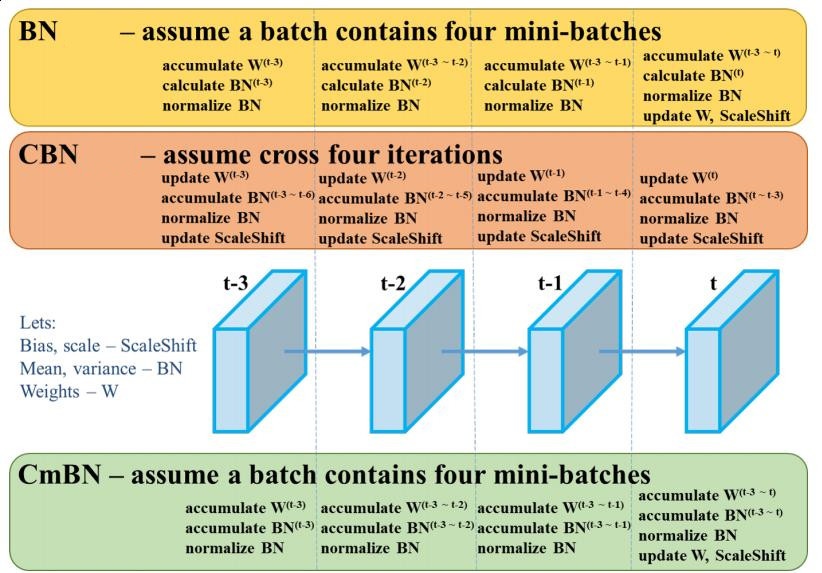
\includegraphics[width=0.7\textwidth]{cmbn}
	\caption[]{Cross Mini Batch Normalization}
  \label{}
\end{figure}

Cross mini Batch Normalisation is used. It is a modified Cross Batch Normalization (CmBN). CmBN collects statistics only between mini-batches within a single batch. 

SAM is modified from spatial-wise attention to point-wise attention (figure~\ref{fig:SAM}), and the shortcut connection in PAN are replaced to concatenation, as can be seen in figure~\ref{fig:PAN}

\begin{figure}[H]
     \centering
     \begin{subfigure}[b]{0.4\textwidth}
         \centering
         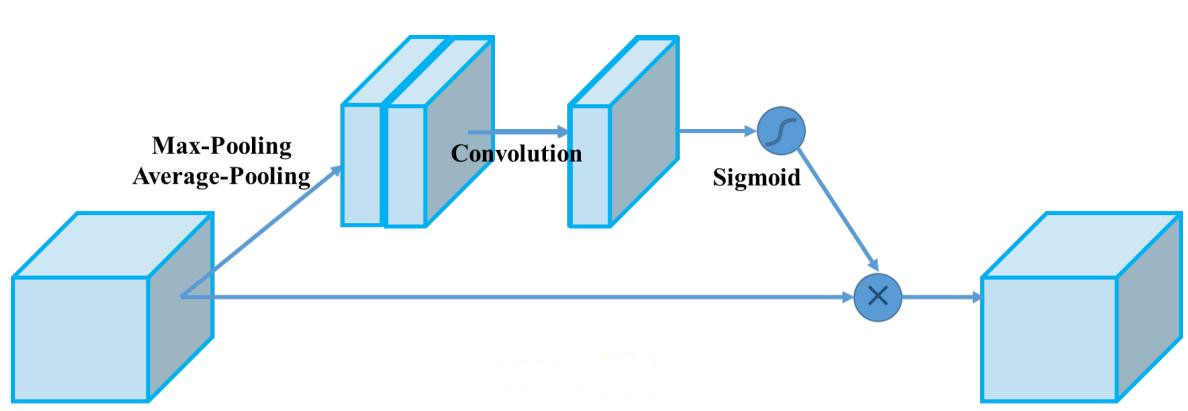
\includegraphics[width=\textwidth]{sam}
         \caption{SAM}
         \label{fig:samnorm}
     \end{subfigure}
     \begin{subfigure}[b]{0.4\textwidth}
         \centering
         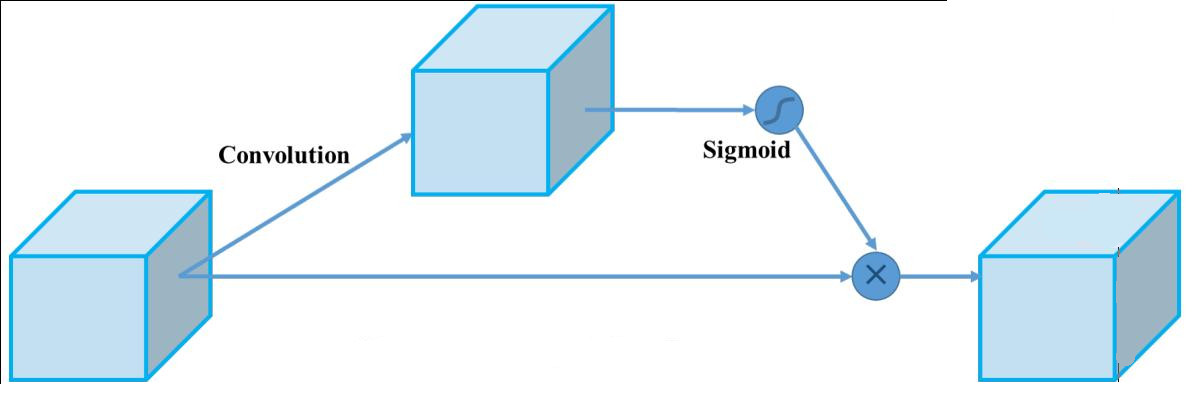
\includegraphics[width=\textwidth]{samMod}
         \caption{Modified SAM}
         \label{fig:samod}
     \end{subfigure}
   \caption{SAM and its YOLO modification}
  \label{fig:SAM}
\end{figure}

\begin{figure}[H]
     \centering
     \begin{subfigure}[b]{0.3\textwidth}
         \centering
         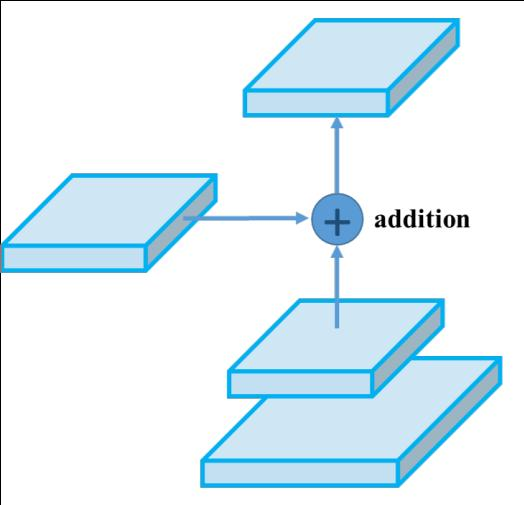
\includegraphics[width=\textwidth]{pan}
         \caption{PAN}
         \label{fig:pan}
     \end{subfigure}
     \begin{subfigure}[b]{0.3\textwidth}
         \centering
         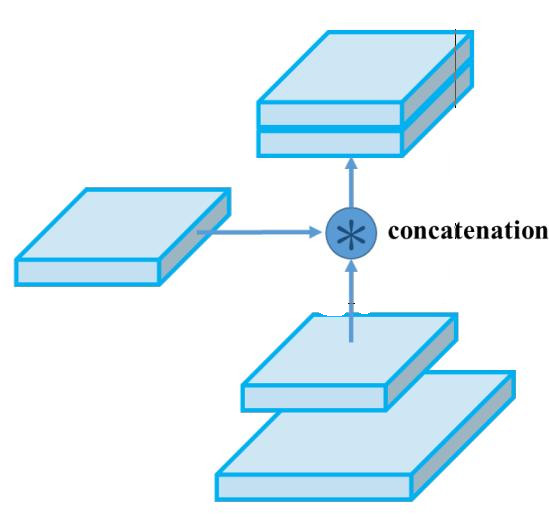
\includegraphics[width=\textwidth]{panMod}
         \caption{Modified PAN}
         \label{fig:panmod}
     \end{subfigure}
   \caption{PAN and its YOLO modification}
   \label{fig:PAN}
\end{figure}
\subsection{YOLOv4 Architecture}
YOLOv4 basic architecture is as follows:
\begin{itemize}
	\item \textbf{Backbone}CSPDarknet53\cite{CSPDarknet53}
	\item \textbf{Neck}: SPP, PAN
	\item \textbf{Head}: YOLOv4
\end{itemize}

 
For the backbone, YOLOv4 uses the following "Bag of Freebies": CutMix and Mosaic Data Augmentation, DropBlock regularization and Class label smoothing. The bag of Specials are Mish Activation, Cross-stage partial connections (CSP) and multi-input weighted residual connections (MiWRC).

For the detector, YOLOv4 uses these "Bag of Freebies": CIoU-loss, CmBn, DropBlock Regularization, Mosaic Data augmentation, Self-Adversarial Training, elimination of grid sensitivity, usage of multiple anchors for a single ground truth, a cosine annealing scheduler \cite{cosineSchedule}, optimal hyper-parameters and random training shapes. These Bag of Specials are used: Mish Activation, SPP-block, SAM-block, PAN Path-aggragation block, DIoU-NMS.

\subsection{Results}
\subsubsection{Influence of features on Classifier training}
The authors studies the influence of different data augmentation techniques, such as bilateral blurring, MixUp, CutMix and Mosaic, along with the influence of different activations like Leaky-ReLU, Swish and Mish.

Table~\ref{tab:cspResNextFeatures} shows the results of those tests for the CSPResNext-50 backbone, and Table \ref{tab:CSPDarknet53} for the CSPDarknet-53 backbone. The classifier accuracy is improved by introducing the CutMix and Mosaic data augmentation, Class label smoothing and the Mish activation. 

\begin{table}[h!]
	\centering
	\begin{tabular}{@{}lllllllll@{}}
		\toprule
		MixUp      & CutMix     & Mosaic     & Bluring    & Label Smoothing & Swish      & Mish       & Top-1           & Top-5           \\ \midrule
		&            &            &            &                 &            &            & 77.9\%          & 94.0\%          \\ \midrule
		\checkmark &            &            &            &                 &            &            & 77.2\%          & \textbf{94.0\%} \\
		& \checkmark &            &            &                 &            &            & \textbf{78.0\%} & \textbf{94.3\%} \\
		&            & \checkmark &            &                 &            &            & \textbf{78.1\%} & \textbf{94.5\%} \\
		&            &            & \checkmark &                 &            &            & 77.5\%          & 93.8\%          \\
		&            &            &            & \checkmark      &            &            & \textbf{78.1\%} & \textbf{94.4\%} \\
		&            &            &            &                 & \checkmark &            & 64.5\%          & 86.0\%          \\
		&            &            &            &                 &            & \checkmark & \textbf{78.9\%} & \textbf{94.5\%} \\
		& \checkmark & \checkmark &            & \checkmark      &            &            & \textbf{78.5\%} & \textbf{94.8\%} \\
												   & \checkmark & \checkmark &            & \checkmark      &            & \checkmark & \textbf{79.8\%} & \textbf{95.2\%} \\ \bottomrule
	\end{tabular}
												   \caption{Impact of Bag of Freebies and different activation on the CSPResNext-50 Classifier. Baseline is shown on the first row. Results which are better than the baseline are shown in bold}
												   \label{tab:cspResNextFeatures}
\end{table}

\begin{table}[h!]
	\centering
	\begin{tabular}{@{}lllllllll@{}}
		\toprule
		MixUp & CutMix     & Mosaic     & Bluring & Label Smoothing & Swish & Mish & Top-1  & Top-5  \\ \midrule
		&            &            &         &                 &       &      & 77.2\% & 93.6\% \\ \midrule
		& \checkmark & \checkmark &         & \checkmark      &       &      & \textbf{77.8\%} & \textbf{94.4\%} \\
		  & \checkmark & \checkmark &         & \checkmark      &       &      & \textbf{78.7\%} & \textbf{94.8\%} \\ \bottomrule
	\end{tabular}
		  \caption{Impact of Bag of Freebies and Mish on the CSPDarknet-53 Classifier. Baseline is shown on the first row. Results which are better than the baseline are shown in bold}
		  \label{tab:CSPDarknet53}
\end{table}

\subsubsection{Influence of features on the Detector training}
In order to better understand the impact of different Bag-of-Freebies on the detector training accuracy, the authors studies different features that increase the detector accuracy without affecting the FPS.

\begin{itemize}
	\item \textbf{S} -  Elimination of grid sensitivity. In YOLOv3, the equation $b_x = \sigma(t_x) + c_x, b_y = \sigma(t_y) + c_y$, with $c_x, c_y$ being whole numbers is used to evaluate the object coordinates. Very high absolute values of $t_x$ are needed for the $b_x$ value to approach $c_x$ or $c_x + 1$. This problem is solved by multiplying the sigmoid by a factor exceeding 1.0, eliminating the effect of grid on which the object is undetectable.
	\item \textbf{M}: Mosaic data augmentation - using the 4-image mosaic during training instead of a single image
	\item \textbf{IT}: IoU thresholding - Using multiple anchors for a single ground truth with $IoU(truth, anchor) > IoU_{threshold}$
	\item \textbf{GA}: Genetic Algorithms - Using genetic algorithms to select the optimal hyperparameters during network training 
	\item \textbf{LS}: Class label smoothing - using class label smoothing for sigmoid activation
	\item \textbf{CBN}: CmBN - using Cross mini-Batch Normalization for collecting statistics inside the entire batch instead of inside a single mini-batch
	\item \textbf{CA}: Cosine annealing scheduler - altering the learning rate following a cosine
	\item \textbf{DM}: Dynamic mini-batch size - automatic increase of mini-batch size during small resolution training by using random training shape
	\item \textbf{OA}: Optimized Anchors - using the optimized anchors for training with $512 \times 512$ network resolution
	\item \textbf{GIoU, CIoU, DIoU, MSE}: Using different loss algorithms for bounded box regression
\end{itemize}

An ablation studies using those bag of freebies is shown in table \ref{tab:bofDetector}


% Please add the following required packages to your document preamble:
% \usepackage{booktabs}
\begin{table}[]
	\centering
	\begin{tabular}{@{}lllllllllllll@{}}
		\toprule
		\textbf{S} & \textbf{M} & \textbf{IT} & \textbf{GA} & \textbf{LS} & \textbf{CBN} & \textbf{CA} & \textbf{DM} & \textbf{OA} & \textbf{Loss} & \textbf{AP}     & \textbf{$AP_50$}  & \textbf{$AP_75$}  \\ \midrule
		           &            &             &             &             &              &             &             &             & MSE           & 38.0\%          & 60.0\%          & 40.8\%          \\ \midrule
			   \checkmark &            &             &             &             &              &             &             &             & MSE           & 37.7\%          & 59.9\%          & 40.5\%          \\
			              & \checkmark &             &             &             &              &             &             &             & MSE           & \textbf{39.1\%} & \textbf{61.8\%} & \textbf{42.0\%} \\
				                 &            & \checkmark  &             &             &              &             &             &             & MSE           & 36.9\%          & 59.7\%          & 39.4\%          \\
						            &            &             & \checkmark  &             &              &             &             &             & MSE           & \textbf{38.9\%} & \textbf{61.7\%} & \textbf{41.9\%} \\
							               &            &             &             & \checkmark  &              &             &             &             & MSE           & 33.0\%          & 55.4\%          & 35.4\%          \\
								                  &            &             &             &             & \checkmark   &             &             &             & MSE           & \textbf{38.4\%} & \textbf{60.7\%} & \textbf{41.3\%} \\
										             &            &             &             &             &              & \checkmark  &             &             & MSE           & \textbf{38.7\%} & \textbf{60.7\%} & \textbf{41.9\%} \\
											                &            &             &             &             &              &             & \checkmark  &             & MSE           & 35.3\%          & 57.2\%          & 38.0\%          \\
													\checkmark &            &             &             &             &              &             &             &             & GIoU          & \textbf{39.4\%} & 59.4\%          & \textbf{42.5\%} \\
													\checkmark &            &             &             &             &              &             &             &             & DIoU          & \textbf{39.1\%} & 64.0\%          & \textbf{44.8\%} \\
													\checkmark &            &             &             &             &              &             &             &             & CIoU          & \textbf{39.6\%} & 59.2\%          & \textbf{42.6\%} \\
													\checkmark & \checkmark & \checkmark  & \checkmark  &             &              &             &             &             & CIoU          & \textbf{41.5\%} & \textbf{64.0}\%          & \textbf{44.8\%} \\
													           & \checkmark &             & \checkmark  &             &              &             &             & \checkmark  & CIoU          & 36.1\%          & 56.5\%          & 38.4\%          \\
														   \checkmark & \checkmark & \checkmark  & \checkmark  &             &              &             &             & \checkmark  & MSE           & \textbf{40.3\%}          & \textbf{64.0\%} & \textbf{43.1\%} \\
														   \checkmark & \checkmark & \checkmark  & \checkmark  &             &              &             &             & \checkmark  & GIoU          & \textbf{42.4\%}         & \textbf{64.4\%} & \textbf{45.9\%} \\
														   \checkmark & \checkmark & \checkmark  & \checkmark  &             &              &             &             & \checkmark  & CIoU          & \textbf{42.4\%}         & \textbf{64.4\%} & \textbf{45.9\%} \\ \bottomrule
	\end{tabular}
	\caption{Ablation Studies of Bag-of-Freebies using CSPResNeXt50-PANet-SPP with $512 \times 512$ input. Baseline is shown on the first row. Results better than baseline are shown in bold.}
	\label{tab:bofDetector}
\end{table}

\subsection{Influence of different backbones and pre-trained weights on the detector}

The authors conducted another study, where they measured the performance of different backbones with the same training parameters, which is reproduced on table \ref{tab:detectorTraining}. It is apparent that \textbf{the model with the best classification accuracy is not always the best in terms of detector accuracy}. CSPResNeXt-50 models trained with different features obtain better classification accuracy, CSPDarknet53 obtains a higher accuracy in the object detection task.

Using BoF and Mish activations for the CSPResNeXt50 classifier increases its classification accuracy but further application of the pre trained weights reduces the detector accuracy. This is not true for CSPDarknet53: with the applications of BoF and Mish increasing both the detector and classifier accuracy. Considering those results, it would seem that \textbf{CSPDarknet53 is more suitable for the detector.}

\begin{table}[h!]
	\centering
	\begin{tabular}{@{}lllll@{}}
		\toprule
		\textbf{Model (with optimal settings)}                                                 & \textbf{Input Size} & \textbf{AP} & \textbf{$AP_50$} & \textbf{$AP_75$} \\ \midrule
		CSPResNeXt50-PANet-SPP                                                                 & $512 \times 512$    & 42.4        & 64.4             & 45.9             \\
		\begin{tabular}[c]{@{}l@{}}CSPResNeXt50-PANet-SPP\\ (BoF-backbone)\end{tabular}        & $512 \times 512$    & 42.3        & 64.3             & 45.7             \\
			\begin{tabular}[c]{@{}l@{}}CSPResNeXt50-PANet-SPP\\ (BoF-backbone + Mish)\end{tabular} & $512 \times 512$    & 42.3        & 64.2             & 45.8             \\ \midrule
				\begin{tabular}[c]{@{}l@{}}CSPDarknet53-PANet-SPP\\ (BoF-backbone)\end{tabular}        & $512 \times 512$    & 42.4        & 64.5             & 46.0             \\
					\begin{tabular}[c]{@{}l@{}}CSPDarknet53-PANet-SPP\\ (BoF-backbone + Mish)\end{tabular} & $512 \times 512$    & 43.0        & 64.9             & 46.5             \\ \bottomrule
	\end{tabular}
	\caption{Comparison study of different classifier pre trained weights for detector trainings.}
	\label{tab:detectorTraining}
\end{table}

\subsubsection{Influence of mini-batch size on detector training}
Finally, the author studied the impact of the mini-batch size on training, which have been reproduced in table \ref{tab:minibatch}

\begin{table}[h!]
	\centering
	\begin{tabular}{@{}lllll@{}}
		\toprule
		\textbf{Model}                                                                                   & \textbf{Input Size} & \textbf{AP} & \textbf{$AP_50$} & \textbf{$AP_75$} \\ \midrule
		\begin{tabular}[c]{@{}l@{}}CSPResNeXt50-PANet-SPP\\ (without BoF/BoS, mini-batch 4)\end{tabular} & $608 \times 608$    & 37.1        & 59.2             & 39.9             \\
			\begin{tabular}[c]{@{}l@{}}CSPResNeXt50-PANet-SPP\\ (with BoF/BoS, mini-batch 8)\end{tabular}    & $608 \times 608$    & 38.4        & 60.6             & 41.6             \\ \midrule
				\begin{tabular}[c]{@{}l@{}}CSPDarknet53-PANet-SPP\\ (without BoF/BoS, mini-batch 4)\end{tabular} & $512 \times 512$    & 41.6        & 64.1             & 45.0             \\
					\begin{tabular}[c]{@{}l@{}}CSPDarknet53-PANet-SPP\\ (with BoF/BoS, mini-batch 8)\end{tabular}    & $512 \times 512$    & 41.7        & 64.2             & 45.2             \\ \bottomrule
	\end{tabular}
	\caption{Comparison study of different mini-batch size for detector training.}
	\label{tab:minibatch}
\end{table}

It seems that that after adding BoF and BoS training strategies, \textbf{the mini-batch size has almost no impact on the detector performance}. This would allow the use of consumer grade GPU to be used to train those detectors, as they would not require as much VRAM for the training.
